\documentclass[aspectratio=169,11pt]{beamer}

\usepackage{fontspec}
\usepackage{polyglossia}
\setdefaultlanguage{romanian}
\setotherlanguage{english}
\defaultfontfeatures{Ligatures=TeX}

\usepackage{amsmath}
\usepackage{booktabs}
\usepackage{graphicx}
\usepackage{array}
\usepackage{xcolor}
\usepackage{tikz}
\usetikzlibrary{arrows.meta,positioning}

\usetheme{Madrid}
\usecolortheme{default}
\setbeamertemplate{navigation symbols}{}
\setbeamertemplate{caption}[numbered]

\definecolor{ubblue}{HTML}{1F4E79}
\definecolor{deepgreen}{HTML}{2E7D5B}
\definecolor{warmgray}{HTML}{4F5B62}
\definecolor{softred}{HTML}{B84A4A}
\definecolor{lightbg}{HTML}{F6F8FA}

\setbeamercolor{structure}{fg=ubblue}
\setbeamercolor{frametitle}{fg=white,bg=ubblue}
\setbeamercolor{title}{fg=white,bg=ubblue}
\setbeamercolor{block title}{fg=white,bg=ubblue}
\setbeamercolor{block body}{bg=lightbg,fg=black}
\setbeamercolor{alerted text}{fg=softred}

\graphicspath{{./}{../}}

\title[Speech Enhancement]{Voice Activity Detection \& Speech Enhancement}
\subtitle{Prezentare lucrare de licență}
\author[Dumitrescu David-Vasile]{Dumitrescu David-Vasile}
\institute[UB FMI]{
  Universitatea din București\\
  Facultatea de Matematică și Informatică\\
  Coordonator științific: Conf. Dr. Cristian Rusu
}
\date{Iunie 2026}

\newcommand{\metric}[2]{\textbf{#1}: \alert{#2}}

\begin{document}

% 1
\begin{frame}
  \titlepage
  \vspace{-0.4cm}
  \begin{center}
    
\includegraphics[height=1.35cm]{assets/logo-ub.png}
    \hspace{1.3cm}
    
\includegraphics[height=1.35cm]{assets/logo-fmi.png}
  \end{center}
\end{frame}

% 2
\begin{frame}{Cuprins}
  \tableofcontents
\end{frame}

\section{Problema abordată și obiectivele proiectului}

% 3
\begin{frame}{Problema abordată}
  \begin{columns}[T,onlytextwidth]
    \column{0.55\textwidth}
      \begin{itemize}
        \item Vorbirea este frecvent afectată de zgomot ambiental.
        \item Problema apare în conferințe online, asistenți vocali, ASR și analiză audio.
        \item Obiectivul este estimarea unui semnal curat, cât mai apropiat de vocea originală.
      \end{itemize}
      \begin{block}{Model aditiv}
        \[
          x[n] = s[n] + v[n]
        \]
        \small
        $s[n]$ - voce curată, $v[n]$ - zgomot, $x[n]$ - semnal observat.
      \end{block}

    \column{0.4\textwidth}
      \centering
      \begin{tikzpicture}[
        signal/.style={
          draw=ubblue,
          rounded corners=2pt,
          align=center,
          minimum width=2.05cm,
          minimum height=0.8cm,
          font=\small
        },
        arrow/.style={-{Latex[length=2mm,width=1.4mm]}, thick, draw=ubblue, shorten >=2pt, shorten <=2pt}
      ]
        \node[signal, fill=deepgreen!12] (speech) at (0,1.0) {Vorbire curată\\$s[n]$};
        \node[signal, fill=softred!12] (noise) at (0,-0.25) {Zgomot\\$v[n]$};
        \node[
          circle,
          draw=ubblue,
          fill=white,
          minimum size=0.48cm,
          inner sep=0pt,
          font=\Large\bfseries
        ] (plus) at (1.85,0.38) {$+$};
        \node[signal, fill=ubblue!10] (noisy) at (3.55,0.38) {Semnal observat\\$x[n]$};

        \draw[arrow] (speech.east) -- (plus.north west);
        \draw[arrow] (noise.east) -- (plus.south west);
        \draw[arrow] (plus.east) -- (noisy.west);

        \node[signal, fill=lightbg, minimum width=2.7cm] (estimate) at (3.55,-1.25) {Estimare\\$\hat{s}[n] \approx s[n]$};
        \draw[arrow] (noisy.south) -- (estimate.north);
      \end{tikzpicture}
      \vspace{0.15cm}

      {\scriptsize Modelul problemei: vocea curată este amestecată cu zgomot, iar sistemul încearcă să recupereze semnalul util.}
  \end{columns}
\end{frame}

% 4
\begin{frame}{Obiective și contribuții}
  \begin{columns}[T,onlytextwidth]
    \column{0.48\textwidth}
      \begin{block}{Obiectiv principal}
        Construirea unui pipeline complet pentru reducerea zgomotului din semnale vocale.
      \end{block}
      \begin{itemize}
        \item pregătire date și mixare controlată;
        \item antrenare MaskNet;
        \item inferență și evaluare obiectivă;
        \item demonstrație real-time.
      \end{itemize}

    \column{0.48\textwidth}
      \begin{block}{Contribuții}
        \begin{itemize}
          \item baseline-uri DSP: Spectral Subtraction și Wiener Filter;
          \item MaskNet cu U-Net rezidual, BiLSTM și attention;
          \item variante IRM și Complex Ratio Mask;
          \item interfață cu forme de undă, spectrograme, VAD și recording.
        \end{itemize}
      \end{block}
  \end{columns}
\end{frame}

\section{Concepte teoretice: STFT, măști spectrale și VAD}

% 5
\begin{frame}{STFT și reconstrucție}
  \begin{columns}[T,onlytextwidth]
    \column{0.52\textwidth}
      \begin{itemize}
        \item Vorbirea este nestaționară, deci este analizată pe cadre scurte.
        \item STFT transformă semnalul din domeniul timp în domeniul timp-frecvență.
        \item ISTFT reconstruiește forma de undă după reducerea zgomotului.
      \end{itemize}
      \begin{block}{Parametri folosiți}
        \begin{itemize}
          \item rată de eșantionare: 16 kHz;
          \item fereastră: 25 ms;
          \item hop: 10 ms;
          \item $NFFT = 512$, rezultând 257 benzi.
        \end{itemize}
      \end{block}

    \column{0.43\textwidth}
      \begin{block}{STFT}
        \[
          X(m,k)=\sum_{n=0}^{L-1}x[n+mH]w[n]e^{-j2\pi kn/N}
        \]
      \end{block}
      \centering
      \begin{tikzpicture}[
        node distance=0.18cm,
        flowbox/.style={
          draw=ubblue,
          rounded corners=2pt,
          align=center,
          minimum width=3.35cm,
          minimum height=0.48cm,
          font=\scriptsize,
          fill=lightbg
        },
        arrow/.style={-{Latex[length=1.8mm]}, thick, draw=ubblue}
      ]
        \node[flowbox] (time) {Semnal în timp\\$x[n]$};
        \node[flowbox, below=of time, fill=deepgreen!10] (stft) {Ferestrare + FFT\\STFT};
        \node[flowbox, below=of stft, fill=ubblue!10] (spec) {Spectrogramă\\$X(m,k)$};
        \node[flowbox, below=of spec, fill=deepgreen!10] (istft) {ISTFT\\semnal reconstruit};

        \draw[arrow] (time) -- (stft);
        \draw[arrow] (stft) -- (spec);
        \draw[arrow] (spec) -- (istft);
      \end{tikzpicture}
  \end{columns}
\end{frame}

% 6
\begin{frame}{Măști spectrale: IRM și CRM}
  \begin{columns}[T,onlytextwidth]
    \column{0.5\textwidth}
      \begin{block}{Ideal Ratio Mask}
        \[
          M_{IRM}=\frac{|X_{clean}|}{|X_{clean}|+|X_{noise}|+\varepsilon}
        \]
      \end{block}
      \begin{itemize}
        \item valori aproape de 1: păstrează energia vorbirii;
        \item valori aproape de 0: atenuează regiunile dominate de zgomot;
        \item formulare stabilă și interpretabilă vizual.
      \end{itemize}

    \column{0.46\textwidth}
      \begin{block}{Complex Ratio Mask}
        \begin{itemize}
          \item folosește partea reală și imaginară a STFT;
          \item permite corecții parțiale ale fazei;
          \item reduce limita impusă de refolosirea fazei zgomotoase.
        \end{itemize}
      \end{block}
      \vspace{0.25cm}
      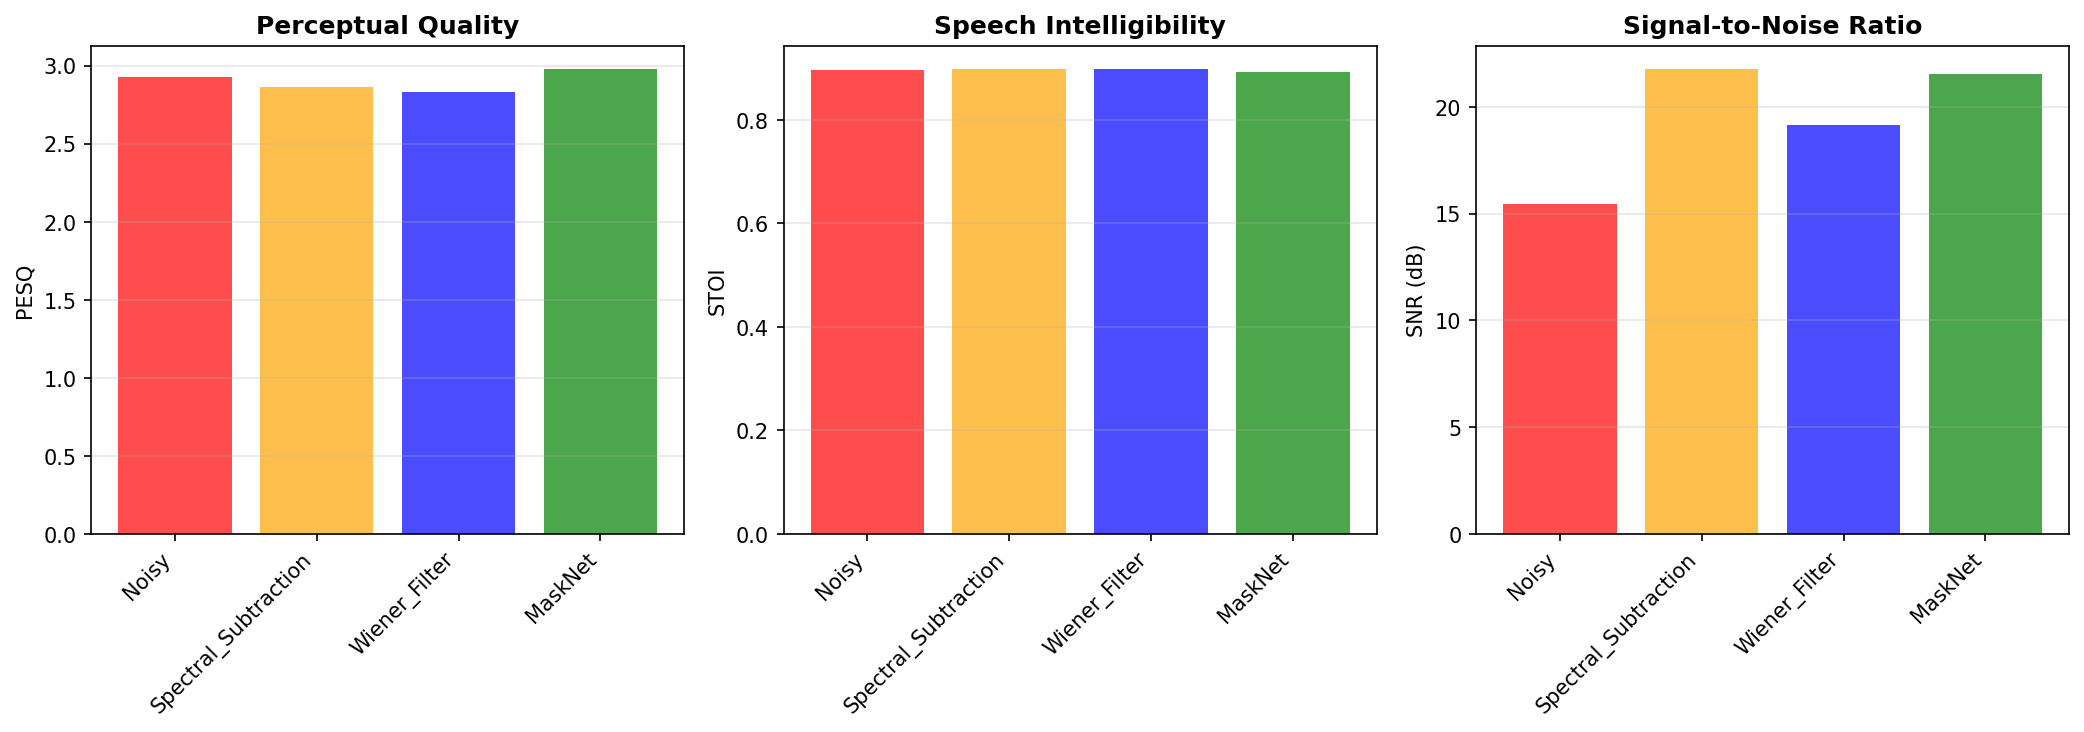
\includegraphics[width=\linewidth]{demo_results/demo_metrics.png}
  \end{columns}
\end{frame}

% 7
\begin{frame}{Voice Activity Detection și metrici}
  \begin{columns}[T,onlytextwidth]
    \column{0.48\textwidth}
      \begin{block}{VAD}
        Identifică segmentele care conțin vorbire și generează etichete hard sau soft.
      \end{block}
      \begin{itemize}
        \item energie;
        \item Zero Crossing Rate;
        \item informație spectrală;
        \item praguri adaptate pentru zone de liniște și vorbire slabă.
      \end{itemize}

    \column{0.48\textwidth}
      \begin{block}{Metrici de evaluare}
        \begin{itemize}
          \item PESQ - calitate perceptuală;
          \item STOI - inteligibilitate;
          \item SNR și segmental SNR;
          \item LSD - distanță spectrală.
        \end{itemize}
      \end{block}
      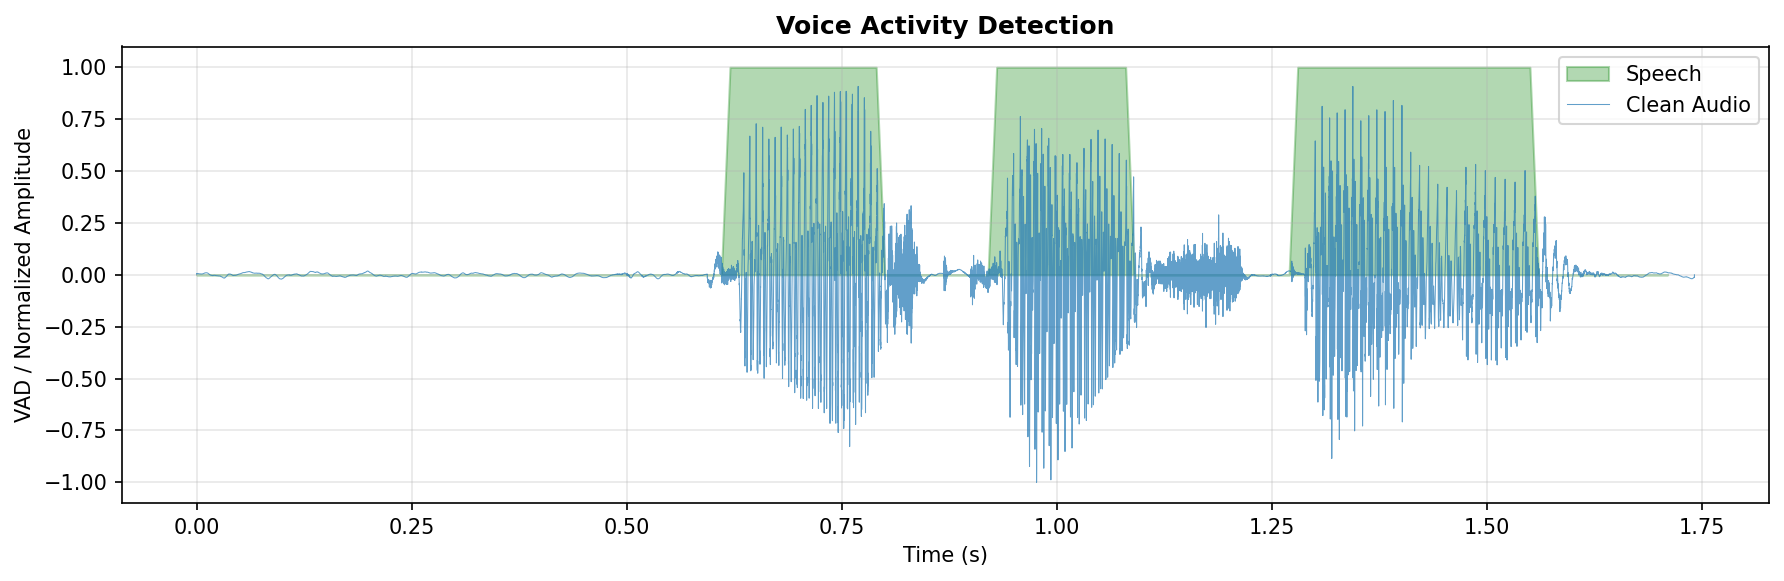
\includegraphics[width=\linewidth]{demo_results/demo_vad.png}
  \end{columns}
\end{frame}

\section{Arhitectura sistemului și modelul MaskNet}

% 8
\begin{frame}{Arhitectura proiectului}
  \begin{columns}[T,onlytextwidth]
    \column{0.48\textwidth}
      \begin{block}{Module principale}
        \begin{itemize}
          \item \texttt{data\_prep}: dataset, validare, augmentare, VAD;
          \item \texttt{dsp}: STFT, ISTFT, metrici și baseline-uri;
          \item \texttt{models}: MaskNet și inferență;
          \item \texttt{train}: antrenare și checkpointing;
          \item \texttt{eval}: rapoarte și grafice;
          \item \texttt{tools}: CLI și demo real-time.
        \end{itemize}
      \end{block}

    \column{0.48\textwidth}
      \begin{block}{Flux general}
        \centering
        Date audio\\
        $\downarrow$\\
        Preprocesare + VAD\\
        $\downarrow$\\
        STFT + model / metodă DSP\\
        $\downarrow$\\
        ISTFT + evaluare + demo
      \end{block}
      \vspace{0.2cm}
      \small
      Separarea modulelor permite reutilizarea aceluiași pipeline în evaluare, demo offline și demo real-time.
  \end{columns}
\end{frame}

% 9
\begin{frame}{Date și antrenare}
  \begin{columns}[T,onlytextwidth]
    \column{0.55\textwidth}
      \begin{itemize}
        \item Antrenare pe LibriSpeech combinat cu zgomote DEMAND.
        \item Mixare on-the-fly la SNR variabil, în intervalul 0-20 dB.
        \item Evaluare finală pe VoiceBank-DEMAND.
        \item Experimentele salvează configurația, istoricul și checkpoint-ul optim.
      \end{itemize}
      \begin{block}{Mixare}
        \[
          x[n] = s[n] + \alpha v[n]
        \]
        \small
        Factorul $\alpha$ este calculat pentru SNR-ul dorit.
      \end{block}

    \column{0.4\textwidth}
      \includegraphics[width=\linewidth]{results/final_report_assets/training_loss_curve.png}
      \vspace{0.1cm}
      {\scriptsize Evoluția funcției de pierdere pentru experimentul final MaskNet.}
  \end{columns}
\end{frame}

% 10
\begin{frame}{Modelul MaskNet}
  \begin{columns}[T,onlytextwidth]
    \column{0.5\textwidth}
      \begin{block}{Configurația recomandată: \texttt{balanced\_res}}
        \begin{itemize}
          \item U-Net rezidual cu patru niveluri encoder-decoder;
          \item skip connections pentru păstrarea detaliilor locale;
          \item BiLSTM pentru context temporal;
          \item Channel Attention pentru ponderarea canalelor.
        \end{itemize}
      \end{block}

    \column{0.46\textwidth}
      \begin{block}{Variante}
        \begin{itemize}
          \item \texttt{tiny}, \texttt{tiny\_fast}: eficiență;
          \item \texttt{balanced\_res}: raport bun calitate-cost;
          \item \texttt{complex\_balanced\_res}: mască complexă;
          \item \texttt{large}, \texttt{xlarge}: calitate, cost mai mare.
        \end{itemize}
      \end{block}
      \begin{block}{Intrare și ieșire}
        Imagine timp-frecvență $\rightarrow$ mască spectrală estimată.
      \end{block}
  \end{columns}
\end{frame}

\section{Demonstrația real-time}

% 11
\begin{frame}{Interfața grafică real-time}
  \begin{columns}[T,onlytextwidth]
    \column{0.62\textwidth}
      \includegraphics[width=\linewidth]{results/realtime_snapshots/realtime_demo_snapshot_20260406_165539.png}

    \column{0.34\textwidth}
      \begin{itemize}
        \item forme de undă raw și enhanced;
        \item spectrograme raw și enhanced;
        \item metode: bypass, Spectral Subtraction, Wiener, MaskNet;
        \item VAD, scenarii, SNR, dry/wet, gain;
        \item snapshot și recording.
      \end{itemize}
  \end{columns}
\end{frame}

% 12
\begin{frame}{Flux real-time și scenarii de test}
  \begin{columns}[T,onlytextwidth]
    \column{0.5\textwidth}
      \begin{block}{Flux audio}
        \centering
        Microfon / speech + noise\\
        $\downarrow$\\
        callback audio rapid\\
        $\downarrow$\\
        coadă de intrare\\
        $\downarrow$\\
        thread de procesare\\
        $\downarrow$\\
        coadă de ieșire + playback
      \end{block}

    \column{0.46\textwidth}
      \begin{block}{Scenarii}
        \begin{itemize}
          \item \texttt{neutral}: mix moderat;
          \item \texttt{office}: EQ și compresie;
          \item \texttt{street}: SNR mai mic, reverb, clipping;
          \item \texttt{hard}: combinație dificilă de distorsiuni.
        \end{itemize}
      \end{block}
      \small
      Compromisul principal este între calitatea procesării și latența acceptabilă în demo.
  \end{columns}
\end{frame}

\section{Rezultate experimentale și concluzii}

% 13
\begin{frame}{Rezultate cantitative}
  \begin{columns}[T,onlytextwidth]
    \column{0.53\textwidth}
      \scriptsize
      \resizebox{\linewidth}{!}{%
      \begin{tabular}{lrrrrr}
        \toprule
        Metoda & PESQ & STOI & SNR & SegSNR & LSD \\
        \midrule
        Noisy & 1.972 & 0.921 & 8.447 & 1.548 & 13.923 \\
        Spectral Subtraction & 2.289 & 0.920 & 10.051 & 3.043 & 11.483 \\
        Wiener Filter & 2.150 & 0.922 & 8.971 & 2.119 & 12.025 \\
        \textbf{MaskNet} & \textbf{2.564} & \textbf{0.929} & \textbf{15.328} & \textbf{6.673} & \textbf{9.502} \\
        \bottomrule
      \end{tabular}
      }

      \vspace{0.25cm}
      \begin{block}{Îmbunătățirea MaskNet față de Noisy}
        \small
        \metric{PESQ}{+0.592} \quad
        \metric{SNR}{+6.882 dB} \quad
        \metric{LSD}{-4.421}
      \end{block}

    \column{0.43\textwidth}
      \includegraphics[width=\linewidth]{results/final_report_assets/final_metrics_comparison.png}
      \vspace{0.1cm}
      \includegraphics[width=\linewidth]{results/final_report_assets/final_improvements.png}
  \end{columns}
\end{frame}

% 14
\begin{frame}{Analiză calitativă, limitări și direcții viitoare}
  \begin{columns}[T,onlytextwidth]
    \column{0.55\textwidth}
      \centering
      \includegraphics[width=\linewidth,height=0.65\textheight,keepaspectratio]{results/final_demo_examples/low_snr/waveforms_spectrograms.png}\par
      \vspace{0.1cm}
      {\scriptsize Exemplu calitativ pentru un caz cu SNR scăzut.}

    \column{0.41\textwidth}
      \footnotesize
      \begin{block}{Interpretare}
        \begin{itemize}
          \item metricile trebuie corelate cu ascultarea exemplelor audio;
          \item spectrogramele evidențiază energia difuză eliminată;
          \item păstrarea formanților indică menținerea detaliilor vocale.
        \end{itemize}
      \end{block}
      \begin{block}{Limitări și direcții}
        \begin{itemize}
          \item estimarea fazei;
          \item costul real-time;
          \item date de antrenare mai diverse;
          \item export ONNX și pierderi perceptuale.
        \end{itemize}
      \end{block}
  \end{columns}
\end{frame}

% 15
\begin{frame}{Concluzii și demo live}
  \begin{columns}[T,onlytextwidth]
    \column{0.55\textwidth}
      \begin{block}{Concluzie}
        Proiectul realizează un sistem complet de Speech Enhancement, combinând metode DSP, rețele neuronale MaskNet, VAD, evaluare obiectivă și demonstrație real-time.
      \end{block}
      \begin{itemize}
        \item MaskNet obține cea mai bună îmbunătățire globală.
        \item Interfața real-time face diferențele vizibile și audibile.
        \item Pipeline-ul este modular și reproductibil.
      \end{itemize}

    \column{0.4\textwidth}
      \centering
      \vspace{0.6cm}
      {\Huge Întrebări?}

      \vspace{0.8cm}
      {\Large Demo real-time}
  \end{columns}
\end{frame}

\end{document}
